\documentclass[notitlepage,a4paper,fleqn,9pt]{extarticle}
%\documentclass[notitlepage,a4paper,fleqn,9pt]{article}

\usepackage{ifluatex}
\ifluatex
  \usepackage{fontspec}
  %\setmainfont[Ligatures=TeX]{xits}
  %\setmainfont[Ligatures=TeX]{Latin Modern Roman}
  %\fontspec[SmallCapsFeatures={Letters=SmallCaps}]{Latin Modern Roman}
  \setmainfont[
    BoldFont={TeX Gyre Termes Bold},
    ItalicFont={TeX Gyre Termes Italic},
    BoldItalicFont={TeX Gyre Termes Bold Italic},
    Ligatures=TeX,
    SmallCapsFeatures={Letters=SmallCaps}
    ]{TeX Gyre Termes}

% \setmainfont[
%  Ligatures=TeX
%  BoldFont={Minion Pro Bold},
%  ItalicFont={Minion Pro Italic},
%  BoldItalicFont={Minion Pro Bold Italic}
%  ]{Linux Libertine O}

\else
  \usepackage[utf8]{inputenc}
  \usepackage[T1]{fontenc}
  \usepackage{times}
\fi

\usepackage{amsmath}
\usepackage{fancyhdr}
\usepackage{indentfirst}
%\usepackage{times}
\usepackage{graphicx}
%\usepackage[dvips]{graphicx}
\usepackage{multicol}
\usepackage{here}

%\usepackage[latin2]{inputenc}

%-----------------------------------------------------------------------------
%\usepackage{psfig}
%\newcommand{\PSFIG}[1]{\psfig{#1}}
%\newcommand{\PSFIG}[1]{}
%-----------------------------------------------------------------------------

\topmargin=-10mm \headsep=5mm \evensidemargin=-12mm
\oddsidemargin=-6mm \textwidth=170mm \textheight=242mm
\columnsep=6mm

\pagestyle{fancy}
\renewcommand{\headrulewidth}{0.1pt}
\fancyhf{} \fancyhead{ {\textbf{CMM-2013} -- Computer Methods
in Mechanics \hfill  27--31 August 2013, Poznan, Poland} }
\fancypagestyle{plain}

\setlength{\arrayrulewidth}{0.1pt}
\setlength{\parindent}{0.5cm}
\mathindent0cm

\makeatletter
\renewcommand{\@seccntformat }[1]{\csname the#1\endcsname.\quad}
\renewcommand\section{\@startsection {section}{1}
{-\parindent}{3ex \@plus -1ex \@minus -.2ex}
{3ex \@plus -1ex \@minus -.2ex}{\textbf}}
\renewcommand\subsection{\@startsection {subsection}{2}
{-\parindent}{1.5ex \@plus -1ex \@minus -.2ex}
{1.5ex \@plus -1ex \@minus -.2ex}{\textit}}

\long\def\@makecaption#1#2{%
  \vskip\abovecaptionskip
  \sbox\@tempboxa{#1: #2}%
  \ifdim \wd\@tempboxa >\hsize
    #1: #2\par
  \else
    \global \@minipagefalse
    \hb@xt@\hsize{\box\@tempboxa}%
  \fi
  \vskip\belowcaptionskip}

\renewcommand\maketitle{\par
  \begingroup
    \renewcommand\thefootnote{\@fnsymbol\c@footnote}%
    \def\@makefnmark{\rlap{\@textsuperscript{\normalfont\@thefnmark}}}%
    \long\def\@makefntext##1{\parindent 1em\noindent
%            \hb@xt@1.8em{%
            \hb@xt@0.5em{%
                \hss\@textsuperscript{\normalfont\@thefnmark}}##1}%
    \if@twocolumn
      \ifnum \col@number=\@ne
        \@maketitle
      \else
        \twocolumn[\@maketitle]%
      \fi
    \else
      \newpage
      \global\@topnum\z@   % Prevents figures from going at top of page.
      \@maketitle
    \fi
    \thispagestyle{plain}\@thanks
  \endgroup
  \setcounter{footnote}{0}%
  \global\let\thanks\relax
  \global\let\maketitle\relax
  \global\let\@maketitle\relax
  \global\let\@thanks\@empty
  \global\let\@author\@empty
  \global\let\@date\@empty
  \global\let\@title\@empty
  \global\let\title\relax
  \global\let\author\relax
  \global\let\date\relax
  \global\let\and\relax
}
\makeatother

\renewcommand{\footnoterule}
  {\noindent\rule{\textwidth}{0.1pt}\vspace{1mm}}
\renewcommand{\baselinestretch}{0.913}


%\usepackage{microtype}
\usepackage{contmech}
\usepackage{tikz}
\usepackage{pgfplots}
\pgfplotsset{compat=newest}

\ifluatex
  \usepackage{unicode-math}
  %\setmathfont[math-style=ISO]{xits-math.otf}
  %\setmathfont[math-style=ISO]{Asana-Math.otf}
1  \setmathfont[math-style=ISO]{latinmodernmath-regular.otf}
  %\setmathfont[math-style=ISO]{texgyretermes-regular.otf}
  \renewcommand{\ta}[1]{\mathbfit{#1}}
  \renewcommand{\ts}[1]{\mathbfit{#1}}
  \renewcommand{\td}[1]{\mathbfcal{#1}}
  \renewcommand{\tf}[1]{\mathbfsfup{#1}}
  \renewcommand{\diff}{\mathbfup{\nabla}}
  \renewcommand{\Box}{\mdlgwhtsquare}
  \renewcommand{\leadsto}{\rightsquigarrow}
\fi


\newcommand{\ded}{\mathrm{d}}
\newcommand{\dep}{\mathrm{p}}
\newcommand{\derv}{\mathrm{v}}
\newcommand{\volume}{\frac{1}{|\Omega_\Box|}}
\newcommand{\jump}[1]{[\![#1]\!]}
\newcommand{\Periodic}{\mathrm{P}}

\DeclarePairedDelimiter{\homogenized}{\langle}{\rangle}
\newcommand{\pore}{\mathrm{pore}}
\newcommand{\particle}{\mathrm{part}}
\newcommand{\contact}{\mathrm{cont}}
\newcommand{\surf}{\mathrm{s}}
\newcommand{\on}{\quad\text{ on }}
\newcommand{\NDIM}{n_\mathrm{dim}}
\newcommand{\tang}{\mathrm{T}}

\newcommand{\figref}[1]{Fig.~\ref{#1}}


\title{\bfseries
On the formulation of a computational homogenization scheme with seamless transition from compressible to incompressible microstructures.
%Boundary conditions and bounds for computational homogenization of incompressible microstructures
}

\author{\normalsize\bfseries
Mikael Öhman$^1$ and Kenneth Runesson$^2$ and Fredrik Larsson$^3$
%\footnote{ Footnotes may appear on the first page only to indicate research grant, sponsoring agency, etc. These should not be numbered but referred to by symbols, e.g. *,+. The footnote text may be produced in a small font. }
}
\date{\normalsize\vspace{-2ex}\em
$^1$Department of Applied Mechanics, Chalmers University of Technology\\
Hörsalsvägen 7, Göteborg, Sweden\\
e-mail: mikael.ohman@chalmers.se\\[1.1mm]
%
$^2$Department of Applied Mechanics, Chalmers University of Technology\\
Hörsalsvägen 7, Göteborg, Sweden\\
e-mail: kenneth.runesson@chalmers.se\\[1.1mm]
%
$^3$Department of Applied Mechanics, Chalmers University of Technology\\
Hörsalsvägen 7, Göteborg, Sweden\\
e-mail: fredrik.larsson@chalmers.se
}

\begin{document}

\raggedcolumns

\maketitle
\vspace{-3mm}
\noindent\rule{\textwidth}{.1pt}

\noindent
Abstract\\
\vspace{1ex}

\noindent 
% The abstract (max. 10 lines) !!!!
In this work, we show the classical boundary conditions in computational homogenization, Dirichlet and Neumann, applied to the case of incompressible microstructures.
We adopt a macroscale mixed velocity-pressure formulation that seamlessly handles the transition from compressible to incompressible microstructures.
The application is that of liquid phase sintering, where the microstructure is modeled as a quasistatic mixture of incompressible fluids with pores and surface tension. 
In the case of sintering, the Representative Volume Elements (RVEs) evolves from a porous ``green body'' to a completely dense, and incompressible, microstructure.
The numerical example shows a comparison between the Dirichlet and Neumann type boundary conditions on a single unit cell RVE.
\vspace{1ex}

\noindent {\em 
FE2; Multiscale; Neumann boundary conditions; Stokes' flow; Incompressibility; Surface tension; Sintering}

\noindent\rule{\textwidth}{.1pt}
\vspace{2mm}

\begin{multicols}{2}

\section{Introduction}

For many materials with heterogeneous microstructures, computational homogenization has shown to be an effective tool to use.
A prime example of such materials is the so-called ``green body'', a cold compacted metal powder subsequently heated. The surface tension then leads to compaction of the metal particles. 

In Ref.~\cite{Ohman2012a}, we showed how computational homogenization can capture the complex phenomena of compacting particles using Stokes' flow.
However, with traditional homogenization schemes, numerical problems arise when the shear and bulk stiffness differ greatly.
The extreme case is that of an incompressible RVE, which leads to a singular macroscopic problem when formulated in standard fashion.
This problem can be avoided by introducing a weak statement for the volumetric rate of deformation. 
% TODO
%, as shown in Ref.~\cite{Ohman2013a}.
In this contribution, we will compare the use of Dirichlet and Neumann boundary conditions for this new format.
In particular, we aim at establishing bounds of a characteristic RVE-potential based on the choice of boundary conditions.

\section{Macroscale problem}
In order to deal with the transition to incompressibility a mixed velocity-pressure formulation is necessary on the macroscopic level.
%As shown in Ref.~\cite{Ohman2013a}, 
% TODO
It can be shown that the macroscale problem can be written as follows: Find $(\bar{\ta v},\bar p) \in\bar{\set V}\times\bar{\set{P}}$ that solve
%----------------------------------------------------------------------------
\begin{subequations}\label{eq:macro}
\begin{alignat}{3}
 &\int_\Omega \left[\bar{\ts\sigma}_\dev - p\ts I \right]\dprod \left[\delta\bar{\ta v}\outerp \diff\right] \dif v = 0
&\;\;& \forall\; \delta\bar{\ta v} \in \bar{\set{V}}^0
\label{eq:macro_v}
\\
 -&\int_\Omega \left[\bar{\ta v}\cdot\diff - \bar{e} \right] \delta\bar p\dif v = 0 
&\;\;& \forall\; \delta\bar p \in \bar{\set{P}}
 \label{eq:macro_p}
\end{alignat}
\end{subequations}
%----------------------------------------------------------------------------
where $\bar{\ts\sigma}_\dev\{\bar{\ts d}_\dev,\bar p\}$ and $\bar{e}\{\bar{\ts d}_\dev,\bar p\}$ are responses from the RVE-problem in each integration point.
Here the deviatoric and volumetric rate of deformation gradient, $\bar{\ts d}_\dev \defeq \left[\bar{\ta v}\outerp \diff\right]^\sym_\dev$ is introduced.
%----------------------------------------------------------------------------
% The formulation in Eqn. \eqref{eq:macro} allows for seamless transition from macroscopic compressible to incompressible by letting $\bar{c} \to 0$.
% Newton iterations for solving the system in Eqns. \eqref{eq:macro} employ the algorithmic tangents
% %----------------------------------------------------------------------------
% \begin{subequations}\label{eq:macro_sensitivity}
% \begin{align}
%  \dif \bar{\ts\sigma}_\dev &= \bar{\tf E}_\ded \dprod \dif\bar{\ts d}_\dev + \bar{\ts E}_\dep \dif\bar{p}
%  \label{eq:macro_sensitivity_s} \\
%  \dif \bar{e} &= \bar{\ts C}_\ded \dprod \dif \bar{\ts d}_\dev + \bar{C}_\dep \dif\bar{p}
%  \label{eq:macro_sensitivity_e}
% \end{align}
% \end{subequations}


\subsection{RVE problem}
To derive the equations for each type of boundary condition it is convenient to construct a potential from which the Dirichlet and Neumann boundary conditions can be defined as $\inf$-$\sup$ problems.

For an RVE with surface tension and pores, as shown in \figref{fig:initial_rve}, one can show that the suitable RVE potential can be expressed as an implicit function of the macroscopic control variables $\bar{\ts d}_\dev$ and $\bar{p}$:
% TODO
%In order to show the Neumann-type boundary condition we shall first revisit the Dirichlet type boundary condition shown in \cite{Ohman2013a} but expressed as a minimization problem.
% The subscale fluid is still subject to incompressibility constraint
% \begin{gather}
%  \diff \cdot \ta v = 0
% \end{gather}
% and the choice of homogenization of the deviatoric strain rate
% \begin{align}
%  \bar{\ts d}_\dev = \volume\int_{\Gamma_\Box} [\ta v \outerp \ta n]_\dev \dif A
% \end{align}
% In the Dirichlet type boundary condition introduced in \cite{Ohman_etal2012b} the velocity on the boundary was controlled by the prolongated macroscopic deviatoric gradient, $\bar{\ts d}_\dev$, but now we introduce an additional constraint
% \begin{gather}
%  \volume \int_{\Gamma_\Box}[\ta v\outerp\ta n]_\dev \dif A = \bar{\ts d}_\dev
% \end{gather}
% which leads to the suitable general RVE-potential
\begin{multline}
 \Lambda_\Box(\bar{\ts d}_\dev, \bar{p}; \ta v, p, \ta t, \bar{e}) \defeq
     \volume\int_{\Omega_\Box^\particle} \!\!\!\!\![\Psi(\ta v\outerp\diff) - p\;[\ta v\cdot\diff]] \dif V
\\
%   + \volume\int_{\Gamma_\Box^\pore} \hat{\ts\sigma}\dprod[\ta v\outerp\hat{\diff}]\dif A
   + \volume\int_{\Gamma_\Box^\pore} \gamma_\surf \;[\ta v \cdot \hat{\diff}]\dif A
%    + \volume\int_{\Gamma_\Box} [\ta v \cdot \ta n] \dif A \bar{p}
% \\
%    + \left[\bar{\ts d}_\dev - \volume\int_{\Gamma_\Box} [\ta v\outerp\ta n] \dif A\right]\dprod \bar{\ts\sigma}_\dev.
  + \bar{p}\; \bar{e}
\\
  + \volume \int_{\Gamma_\Box^+} \ta t \cdot \jump{[\bar{\ts d}_\dev + \frac13\bar{e}\ts I]\cdot[\ta x - \bar{\ta x}] - \ta v}\dif A
%   + \volume\int_{\Gamma_\Box}[\ta v\cdot \ta n]\dif A\;\bar{p}
%   - \left[\volume \int_{\Gamma_\Box} [\ta v\outerp\ta n]_\dev\dif A - \bar{\ts d}_\dev\right]\dprod \bar{\ts\sigma}_\dev
\label{eq:rve_potential}
\end{multline}
where $\Psi$ is the bulk potential, $\gamma_\surf$ is the surface tension and $\hat{\diff}$ is the surface gradient operator.
The additional field $\ta t$ is the Lagrange multiplier associated with the fluctuations of the velocity on the boundaries of the RVE.

%%%%%%%%%%%%%%%%%%%%%%%%%%%%%%%%%%%%%%%%%%%%%%%%%%%%%%%%%%%%%%%%%%%%%%%%%%%%%%%%%%%%%%%%%%%%%%%%%%%%%%%%%%%%%%%%%%%%%%%%
\subsection{Dirichlet boundary condition}
We can then express the Dirichlet boundary condition as an $\inf$-$\sup$ problem of Eqn.~\eqref{eq:rve_potential} by restricting the space for $\ta v$:
\begin{align}
\label{eq:dirichlet_potential}
 \Psi^\Dirichlet_\Box(\bar{\ts d}_\dev, \bar{p} ) \defeq
    \inf_{\ta v \in \set V_\Box^\Dirichlet } \;
    \sup_{\substack{ p\in \set P_\Box \\ \ta t \in \set{T}_\Box }} \;
    \inf_{\bar{e} \in \set{R}}
    \Lambda_\Box(\bar{\ts d}_\dev, \bar{p}; \ta v, p, \ta t, \bar{e})
\end{align}
where
\begin{align}
 \set{V}_\Box^\Dirichlet =& \{ \ta v \in \set{V}_\Box : \exists\; (\hat{\ts d}_\dev,\bar{e}) \in \set{R}^{3\times 3}_\dev \times \set{R} :
\nonumber\\
  & \ta v = \hat{\ts d}_\dev\cdot[\ta x - \bar{\ta x}] + \bar{e}\;\frac13 [\ta x - \bar{\ta x}] \text{ on }\Gamma_\Box \}
\end{align}
In the Dirichlet boundary condition we solve the sought for volumetric rate of deformation, $\bar{e}$, directly as an unknown in the finite element problem, while the deviatoric stress, $\bar{\ts\sigma}_\dev$ is post-process by homogenization.

%%%%%%%%%%%%%%%%%%%%%%%%%%%%%%%%%%%%%%%%%%%%%%%%%%%%%%%%%%%%%%%%%%%%%%%%%%%%%%%%%%%%%%%%%%%%%%%%%%%%%%%%%%%%%%%%%%%%%%%%
\subsection{Neumann boundary condition}
Similarly, the Neumann boundary condition can be expressed by restricting the space for $\ta t$:
\begin{align}
 \Psi^\Neumann_\Box(\bar{\ts d}_\dev, \bar{p} ) \defeq
    \inf_{\ta v \in \set V_\Box } \;
    \sup_{\substack{p\in \set P_\Box \\ \ta t \in \set T_\Box^\Neumann }} \;
    \inf_{\bar{e} \in \set{R} }
    \Lambda_\Box(\bar{\ts d}_\dev, \bar p; \ta v, p, \ta t, \bar{e})
\end{align}
where
\begin{align}
 \set T_\Box^\Neumann = \{ \ta t : \exists\; (\bar{\ts\sigma}_\dev, \hat{p}) \in \set{R}^{3\times 3}_\dev \times \set{R} : \ta t = \bar{\ts\sigma}_\dev\cdot\ta n - \hat{p}\;\ta n \}
\end{align}
As opposed to the Dirichlet, the deviatoric stress is now solved for directly as an unknown, and the volumetric rate of deformation is post-processed.



%%%%%%%%%%%%%%%%%%%%%%%%%%%%%%%%%%%%%%%%%%%%%%%%%%%%%%%%%%%%%%%%%%%%%%%%%%%%%%%%%%%%%%%%%%%%%%%%%%%%%%%%%%%%%%%%%%%%%%%%
% \subsection{Periodic boundary condition}
% We can express the periodic boundary condition using the same RVE-potential
% \begin{align}
% \label{eq:periodic_potential}
%  \Psi^\Periodic_\Box(\bar{\ts d}_\dev, \bar{p} ) \defeq
%     \inf_{\ta v \in \set V_\Box^\Periodic} \;
%     \sup_{\substack{ p\in \set P_\Box \\ \bar{\ts\sigma}_\dev \in \set{R}_\dev^{3\times 3} }}
%     \Lambda_\Box(\bar{\ts d}_\dev, \bar{p}; \ta v, p, \bar{\ts\sigma}_\dev)
% \end{align}
% where
% \begin{align}
%  \set{V}_\Box^\Periodic =& \{ \ta v \in \set{V}_\Box : \exists\; (\hat{\ts d}_\dev,\bar{e}) \in \set{R}^{3\times 3}_\dev \times \set{R} : 
% \nonumber\\
%     &\jump{\ta v} = \hat{\ts d}_\dev\cdot\jump{\ta x - \bar{\ta x}} + \bar{e}\; \jump{\ta x_\mean} \text{ on }\Gamma_\Box^+ \}.
% \end{align}
% Here we introduced the jump $\jump{\bullet} \defeq \bullet^+ - \bullet^-$, where $+$ and $-$ represents the opposing sides on an cubic RVE.

\section{Numerical examples}

The numerical example shows a comparison of the Dirichlet and Neumann type boundary condition (upper and lower bounds respectively) on a single unit cell RVE.
The unit cell contains 4 particles surrounded by melted binder as seen in \figref{fig:initial_rve}.
The free pore surface is subject to surface tension, which acts as the sole driving force for the simulation, which stops when the pore has vanished.
The RVE's are themselves subject the macroscopic fields $\bar{\ts d}_\dev = \ts 0$ and $\bar{p} = 0$.

\begin{figure}[H]
 \centering
 
\includegraphics[scale=0.25]{figures/initial_rve}
 \caption{Initial state of the RVE with one unit-cell containing stiff particles with soft binder}
 \label{fig:initial_rve}
\end{figure}

In the RVE subject to the Dirichlet boundary condition in \figref{fig:final_dirichlet} we can see a uniform shrinkage on the boundary, as no fluctuations are allowed. 
With the Neumann boundary condition in \figref{fig:final_neumann} we see fluctuations on the boundary where the soft binder, and the hard particles can maintain the initial shape.

\begin{figure}[H]
 \centering
 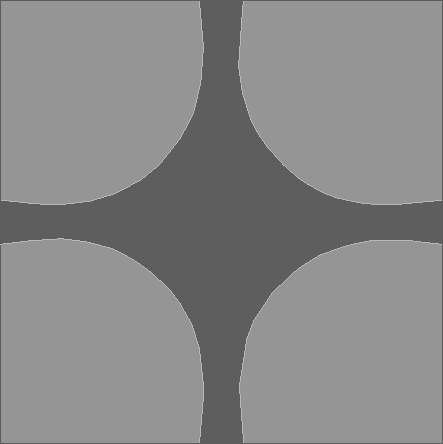
\includegraphics[scale=0.25]{figures/final_dirichlet}
 \caption{Final state of RVE subject to Dirichlet boundary condition}
 \label{fig:final_dirichlet}
\end{figure}

\begin{figure}[H]
 \centering
 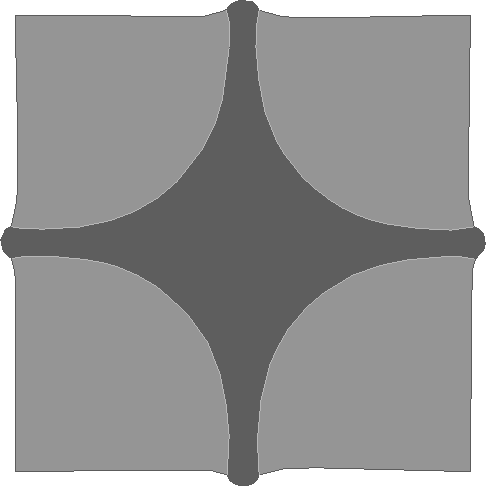
\includegraphics[scale=0.25]{figures/final_neumann}
 \caption{Final state of RVE subject to Neumann boundary condition}
 \label{fig:final_neumann}
\end{figure}

In \figref{fig:porosity} the stiffer solution obtained from the Dirichlet boundary condition shows a clearly slower shrinkage of the RVE, where the pore vanishes after 850 time steps, compared to 715 time steps for the Neumann boundary condition.
We can see in \figref{fig:porosity} that we obtain a tighter bound for the porosity when we increase the RVE size to include multiple unit-cells.

\begin{figure}[H]
 \centering
\begin{tikzpicture}
 \begin{axis}[
    width=1.051\linewidth,
    height=0.7\linewidth,
    ylabel={Porosity [\%]},xlabel={Time steps},
    xmax=1, xmin=0, ymin=-0.01,
    cycle list name=linestyles,
    yticklabel style={font=\small}, xticklabel style={font=\small},
    %scaled y ticks=manual:{}{\pgfmathparse{#1*100}}, % Scale for percentage
    %scaled x ticks=manual:{}{\pgfmathparse{#1*1000}}, % Scale for percentage
    ]
  \addplot[very thick,densely dashed] table {figures/porosity_dirichlet.txt};
  \addlegendentry {Dirichlet}
  \addplot[thick] table {figures/porosity_neumann.txt};
  \addlegendentry {Neumann}

  \addplot[densely dashed] table {figures/porosity_2_dirichlet.txt};
  \addlegendentry {Dirichlet 2$\times$2}
  \addplot[] table {figures/porosity_2_neumann.txt};
  \addlegendentry {Neumann 2$\times$2}

 \end{axis}
\end{tikzpicture}
 \caption{Porosity over time for a single and 2$\times$2 unit-cell RVE subject to zero macroscopic pressure, $\bar{p} = 0$}
 \label{fig:porosity}
\end{figure}

% 
% %%%%%%%%%%%%%%%%%%%%%%%%%%%%%%%%%%%%%%%%%%%%%%%%%%%%%%%%%%%%%%%%%%%%%%%%%%%%%%%%%%%%%%%%%%%%%%%%%%%%%%%%%%%%%
% 
% 
% 
% % The usual text must be written with letter size 9 pt and single
% % spacing. Unless stated otherwise, the font used must be Times-Roman.
% % The words figure, reference and equation have to be abbreviated as
% % Fig. 1, Eqn (\ref{I_formula})  and Ref. \cite{Zienkiewicz00}, unless
% % they appear as the first word of a sentence. In this case they
% % should be typed in full as Figure 1, Equation (\ref{I_formula}) and
% % Reference \cite{Zienkiewicz00}. When a problem is studied in a
% % number of references, one can also refer to them by recalling
% % \cite{AiOd97,AlLaLe98,Zienkiewicz00}.
% 
% \subsection{Figures}
% 
% The name of a figure should appear below it. All figures must be
% numbered sequentially starting with number 1, e.g. Figure 1: Plot of
% a beam eigenfunction $u=u(x)$. Please ensure that all spelling and
% annotations (numbers, letters, symbols and captions) conform to
% their usage in the text. Colour figures cannot be included in their
% original form and will be reproduced in black and white.
% 
% \section{Equations}
% Equations should be placed flush-left with the text margin and
% should be proceeded and followed by a 3 pt vertical space.
% \begin{equation} \label{eqn_in_x}
%   Ax^{2} + Bx + C = 0
% \end{equation}
% 
% \noindent In case of a multiline formula we can write
%   \begin{align}\label{I_formula}
%      I_{\alpha+\beta_i}^j = &\frac{-3}{ac} \left(\sqrt{(a+b)^2+c^2} + \sqrt{(2a-b)^2+c^2} \, + \right.
%    \nonumber \\
%        & \left. + \, \sqrt{(2\beta_i-\alpha)^2+c_j^2} \, \right)
%   \end{align}
% 
%  If the formulae are numbered, make sure that
% they are numbered consecutively. Place the numbers in parentheses
% flush with the right-hand margin of the column and level with the
% last line of the equation. Please ensure that subscripts and
% superscripts are clearly legible. The meaning of the variables used
% should be given or clear from the context.
% 
% \begin{figure}[H]
% \begin{center}
%    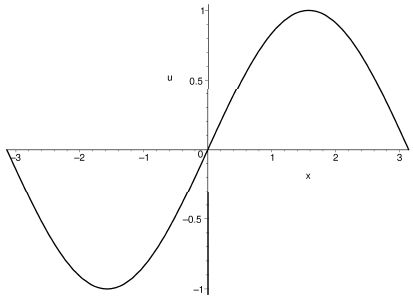
\includegraphics[width=7cm]{figures/plot1}
%    \caption{Plot of a beam eigenfunction $u=u(x)$  }%Figure title
%    \label{fig:lab}
% \end{center}
% \end{figure}
% 

\begin{thebibliography}{99}

\bibitem{Ohman2012a}
   Öhman, M. and Runesson, K. and Larsson, F.,
   Computational Mesoscale Modeling and Homogenization of Liquid-Phase Sintering of Particle Agglomerates,
   \emph{Technische Mechanik},
   32, pp. 463 -- 483, 2012.

% \bibitem{Ohman2013a}
%    Öhman, M. and Runesson, K. and Larsson, F.,
%    Computational Homogenization of Liquid-Phase Sintering with Seamless Transition from Macroscopic Compressibility to Incompressibility,
%    \emph{Computer Methods in Applied Mechanics and Engineering},
%    under review, 2013.

% 
% \bibitem{AlLaLe98}
%   Allix, O., Ladev\`{e}ze, P. and Leveque, D.,
%   Towards a structural identification of delamination initiation and growth,
%   \emph{ ECCM 8: Vol. 1: Composites in aerospace and aeronautics and applications,
%   Proceedings of the 8th European Conference on Composite Materials },
%   Visconti I. C. Ed., Woodhead Publishing Ltd,   Cambridge, Vol. 1, pp. 525-532, 1998.
% 
% \bibitem{Zienkiewicz00}
%    Zienkiewicz, O.C. and Taylor, R.L.,
%    \emph{The Finite Element Method},
%    Vol. 1: \emph{The Basis},
%    fifth ed., Butterworth-Heinemann, Oxford, 2000.

\end{thebibliography}

% The references given above are examples of the following types:
%  1) paper in a journal, 2) paper in a conference
% proceedings, 3) book. References should be collected at the end of
% your paper in alphabetical order according to the numeric sequential
% system. Each item in the list of references should be referred to in
% the text and quoted
%  with numbers enclosed in brackets [1], [2], [3].  The references should be set in the
% following order: author's surname, initials, title, publication,
% volume, page range, year.

\end{multicols}


\end{document}
